% \documentclass[twocolumn]{article}
\documentclass{article}
% \usepackage[a4paper, margin=1in]{geometry} 
\usepackage{graphicx}
\usepackage{subcaption}
\usepackage{amsmath}
\usepackage{hyperref}
\usepackage{float}
\usepackage{algorithm}
\usepackage{algpseudocode}
\usepackage{multirow}

\begin{document}

\title{PA2 report}
\author{Weixiao Zhan}
\date{\today}
\maketitle

\section{Development Flow}

In this project, a general matrix multiplication (GEMM) program
utilizing Compute Unified Device Architecture (CUDA) is implemented
to harvest the computation power and parallel capabilities of Nvidia GPUs.

\subsection{Program}
In short summary, the CUDA GEMM program implemented the routine 
shown in Algorithm \ref{alg:matmul}. 
The program utilized partitioning and pipelining to
achieve significant performance improvement compare to a naive implementation.
\begin{algorithm}
\caption{CUDA GEMM}
\label{alg:matmul}
\begin{algorithmic}[1]
    \State \textbf{Input:} $A,B,C$
    \State Initialize $A\_tile$, $B\_tile$ in shared memory
    \State Initialize $A\_frag$, $B\_frag$, $C\_frag$ in register
    \For {each block tile in $K$ dimension}
        \State Load $A\_tile$ (global $\rightarrow$ shared memory)
        \State Load $B\_tile$ (global $\rightarrow$ shared memory)
        \State Synchronize threads
        \For {each thread tile in the $K$ dimension}
            \State Load $A\_frag$ (shared memory $\rightarrow$ register)
            \State Load $B\_frag$ (shared memory $\rightarrow$ register)
            \State $C\_frag$ += $A\_frag \cdot B\_frag$
        \EndFor
        \State Synchronize threads
    \EndFor
    \State Store $C\_frag$ to $C$ (registers $\rightarrow$ global memory)
\end{algorithmic}
\end{algorithm}


\subsubsection{partition}
\label{sec:partition}
Partition, also called tiling, is one of the most important optimize technique 
for GEMM programs to fully utilize the memory caching hierarchy
and hide memory latency.

Consider matrix multiplication $C = A\cdot B$.
An $O(n^3)$ algorithm would need to load each $A$'s element $N$ times 
and each $B$'s element $M$ times, which, in total, is $2MKN$ times of memory load.
Now suppose, the memory system has caches, i.e. is a two-level system.
The program can rearrange its memory access pattern and reduce the number load from slow memory.

As shown in \ref{fig:partition}, 
the program can place one row partition of A (colored in blue) and 
one column partition of B (colored in green) in fast memory, 
and perform matrix multiplication to get one partition of C (colored in yellow).
In this way, despite the total number of load from fast memory is the same as an naive approach,
the number of load from slow memory is reduced to $MK\cdot \frac{N}{N_{tile}} + KN\cdot\frac{M}{M_{tile}}$

\begin{figure*}[h]
    \centering
    \begin{subfigure}[b]{0.4\linewidth}
        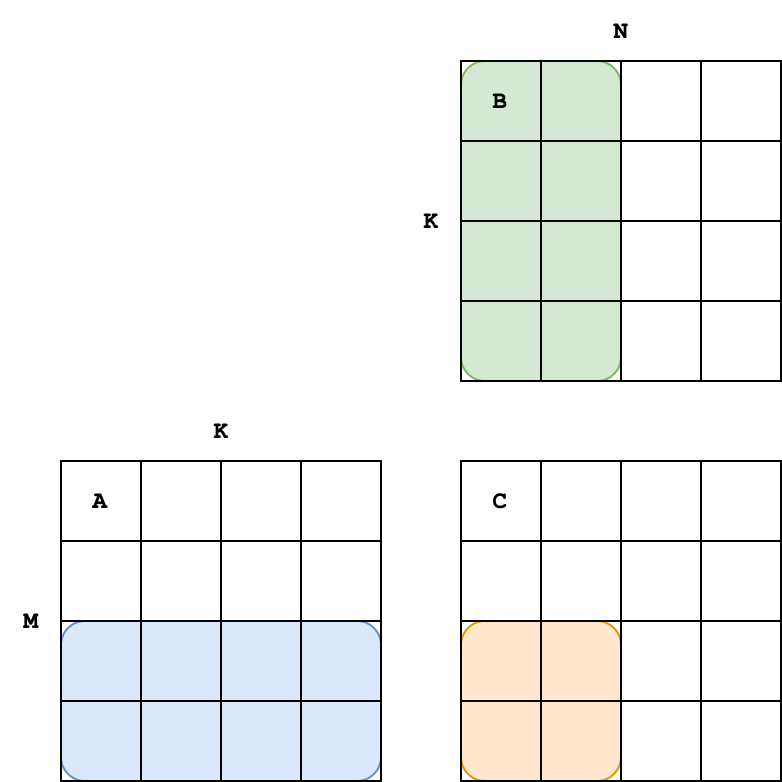
\includegraphics[width=\linewidth]{img/partition.png}
        \caption{consecutive Partition}
        \label{fig:partition}
    \end{subfigure}
    \begin{subfigure}[b]{0.4\linewidth}
        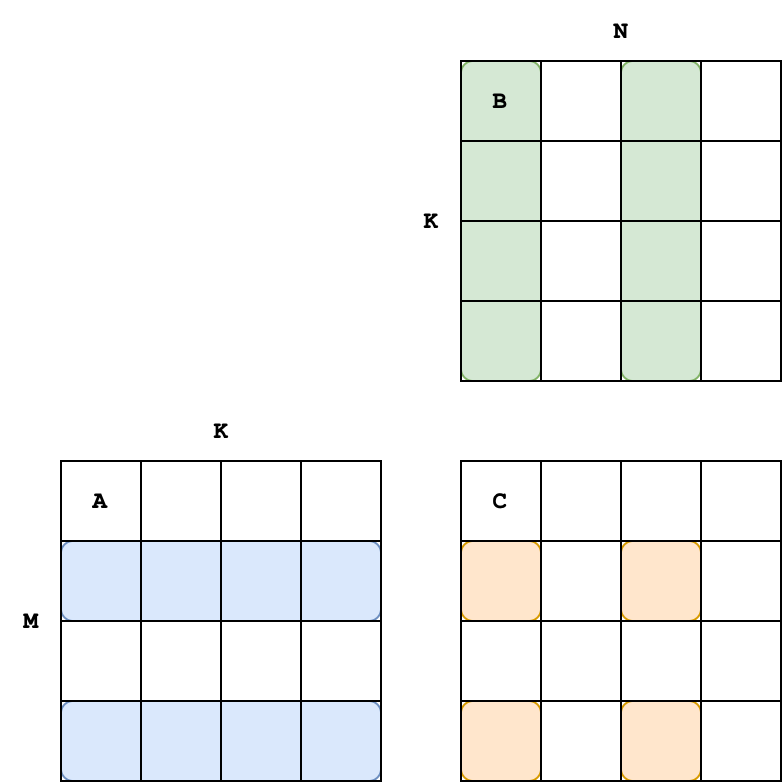
\includegraphics[width=\linewidth]{img/interleave.png}
        \caption{interleaved partition}
        \label{fig:interleave}
    \end{subfigure}
    \caption{partition methods}
\end{figure*}


The partition technique is completable with CUDA paradigm:
there is no dependency between partitions.
Moreover, Nvidia GPUs has a three-level memory hierarchy: global memory, shared memory, registers.
Thus in practice, the partition is also extended to two levels
(shown in Figure \ref{fig:complete-hierarchy}).
Correspondence between GEMM program, CUDA paradigm, and GPU memory hierarchy
is summarized in Table \ref{tab:hierarchy}.
One CUDA grid handles one GEMM with $A$, $B$, and $C$ stored in global memory;
each CUDA block handles one block tile with partitions stored in shared memory;
each CUDA thread handles one thread tile with finer partitions stored in registers.

\begin{figure*}[h]
    \centering
    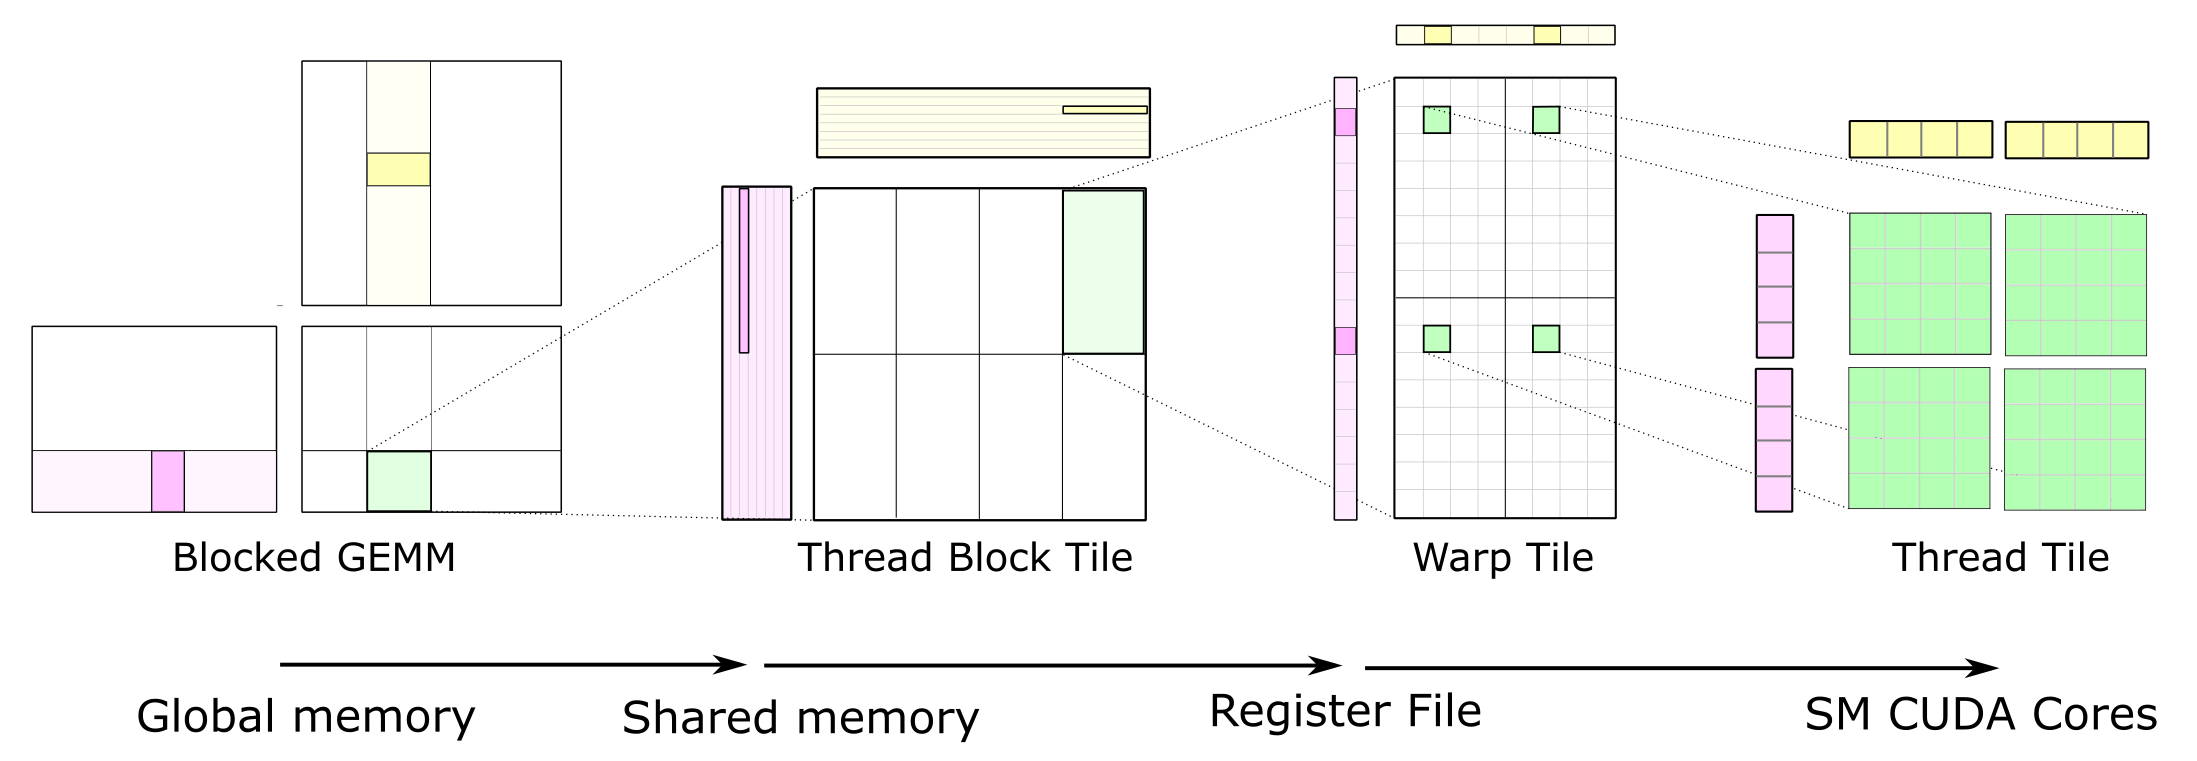
\includegraphics[width=\linewidth]{img/complete-hierarchy.png}
    \caption{CUDA GEMM partition}
    \label{fig:complete-hierarchy}
\end{figure*}


\begin{table}[h]
    \centering
    \begin{tabular}{c|c|c}
    GEMM          & CUDA   & GPU Memory Hierarchy \\ \hline
    entire matrix & grid   & global memory \\
    block tile    & block  & shared memory \\
    thread tile   & thread & registers    
    \end{tabular}
    \caption{Correspondence between GEMM program, CUDA paradigm, and GPU memory hierarchy}
    \label{tab:hierarchy}
\end{table}

\subsubsection{interleave partition}
Nvidia GPU memory supports coalesced loads. 
Thus its beneficial to perform an interleaved partition (shown in \ref{fig:interleave}) 
instead of consecutive partition for thread tile.
With interleaved partition, threads within a block would simultaneously 
perform load operation to adjacent memory locations. 
The GPU would coalesce the loads and maximize the memory bandwidth.

\subsubsection{boundary check}
The size of matrix $A, B$ are not always multiple of block tile sizes.
Thus it is necessary to perform boundary checks to ensure correctness.
In practice, there are two boundary checks are implemented:

\begin{enumerate}
    \item when loading $A\_tile,B\_tile$ from global to shared memory:
    set the shared memory corresponding to out-of-boundary entries to 0;
    \item when storing back $C\_frag$, 
    skip out-of-boundary entries.
\end{enumerate}

Under CUDA paradigm, it is more efficient to 
carry those out-of-boundary entries as zeros
through out the computation instead of using branch statements to identify them.
Branch statements can cause branch divergence and introduce extra cycles.


\subsubsection{software pipelining}
The typical workload paradigm of a CUDA block in our CUDA GEMM program
is shown in Algorithm \ref{alg:workload}.
Note the loads and arithmetic operations are clustered and separated by synchronization barriers. 
Such workload can quickly exhausted the queue of memory unit or arithmetic unit of a streaming multiprocessor (SM),
causing the warp get blocked while the other queue still have capabilities.
when one warp is blocked, 
no other warps from the same CUDA block can make progress on the same SM, 
since they are all waiting for the same resources.
Thus the scheduler can only scheduler warps from another CUDA block and reduce the performance.

The solution is to introducing double caching and software pipelining.
This method can eliminate one synchronization barriers,
as shown in Algorithm \ref{alg:pipeline}.

\begin{figure}[h]
    \centering
    \begin{minipage}{0.47\textwidth}
        \centering
        \begin{algorithm}[H]
            \caption{Workload}
            \label{alg:workload}
            \begin{algorithmic}[1]
                \Repeat
                    \State load one block tile
                    \Comment{many loads}
                    \State synchronize threads
                    \State compute one block tile
                    \Comment{many arithmetic}
                    \State synchronize threads
                \Until{consumed all block tile}
                \State Store register to global memory
            \end{algorithmic}
        \end{algorithm}
    \end{minipage}
    \hspace{0.5cm}
    \begin{minipage}{0.47\textwidth}
        \centering
        \begin{algorithm}[H]
            \caption{Pipelined Workload}
            \label{alg:pipeline}
            \begin{algorithmic}[1]
                \State load one block tile to one cache
                \Repeat
                    \State compute one block tile
                    \State load next block tile to the other cache
                    \State Synchronize threads
                \Until{consumed all block tile}
                \State compute one block tile
                \State Store register to global memory
            \end{algorithmic}
        \end{algorithm}
    \end{minipage}
\end{figure}

\subsection{develop process}
The develop process follows the order below:
\begin{enumerate}
    \item implemented block partition.
    \item implemented boundary check so that the program would work on any size matrices, including non-square ones.
    \item implemented thread interleaved partition, 
    allowing each thread processing multiple entire.
    \item implemented pipelining.
    \item implemented auto-tuning Python script \texttt{auto.py} to search best tile sizes for different matrix sizes.
\end{enumerate}


\subsection{incremental improvement}
As shown in Figure \ref{fig:develop-process}, 
partition (block tiles), interleaved partition (thread tiles), pipelining, and parameter tuning 
give incremental performance improvement;
meanwhile the necessary boundary checks costed negligible performance loss.
In sum, all optimization methods are working.

\begin{figure*}[h]
    \centering
    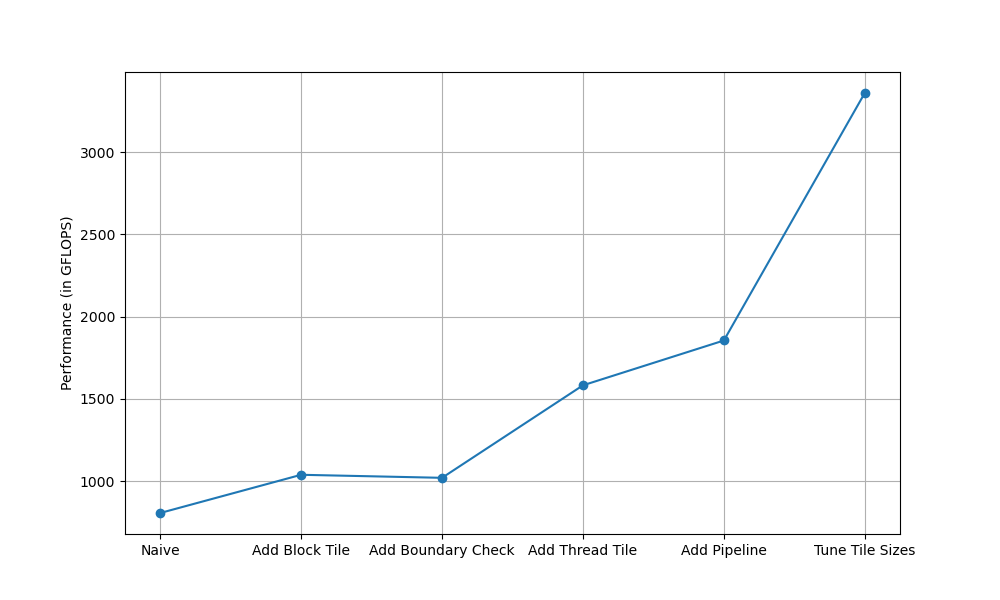
\includegraphics[width=\linewidth]{img/develop_process.png}
    \caption{performance gain during develop process on $n=1024$}
    \label{fig:develop-process}
\end{figure*}

\newpage
\section{Result}

The auto-tuning script explored block tile sizes
\footnote{block tile size refer to the number entries processed by one CUDA block}
$Bs = \{16, 32, 64\}$
and thread tile sizes 
\footnote{thread tile size refer to the number entries processed by one CUDA thread}
$Ts = \{1,2,4,8\}$
on problem sizes $n = \{128^{\ddagger} , 256^{\ddagger}, 512^{\ddagger}, 768^{\ddagger}, 1024^{\ddagger}, 2048^{\ddagger} 4096^{\ddagger}\}$
\footnote{$n^{\ddagger} = \{n-1, n, n+1\}$}.
The results are present in \texttt{resutls.csv}.

Figure \ref{fig:result} shows the best performing 4 tile size combinations out of the 12 been measured.
\begin{figure*}[h]
    \centering
    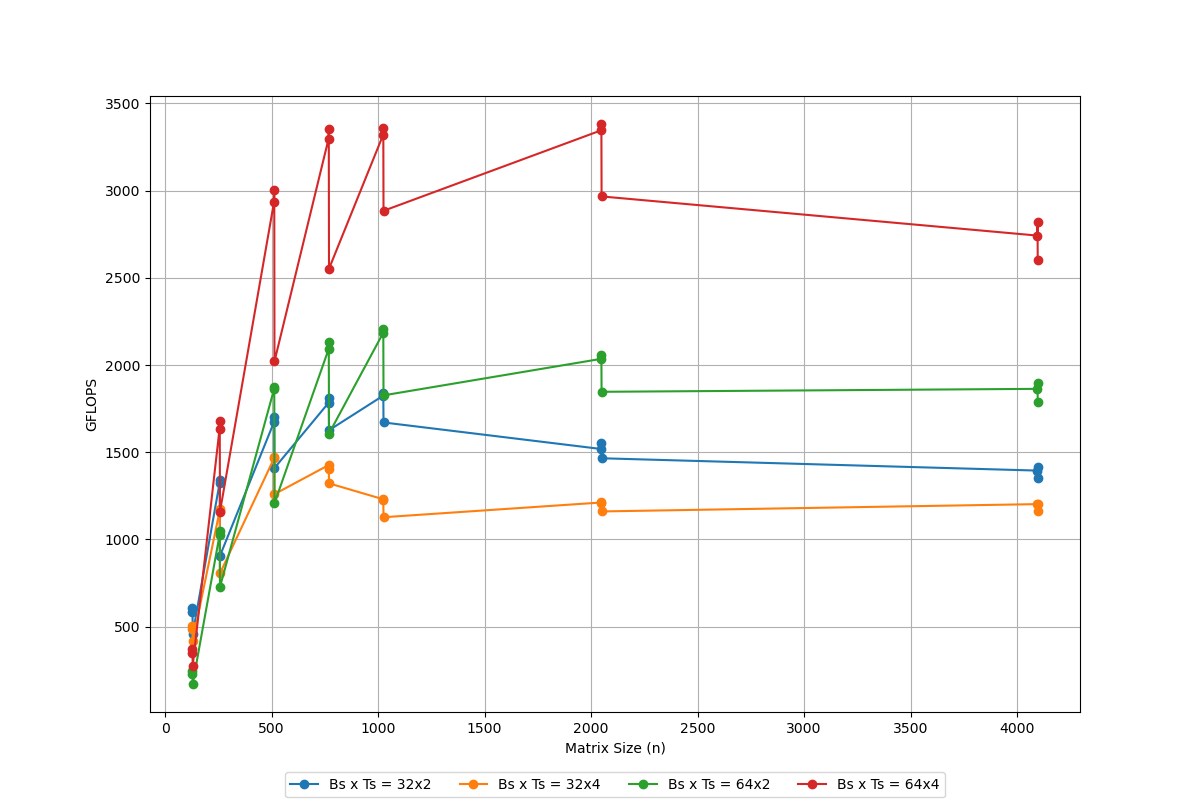
\includegraphics[width=\linewidth]{img/result.png}
    \caption{performance}
    \label{fig:result}
\end{figure*}

\subsection{tile size limitation}
Denote the block tile size $B_s$ and thread tile size $T_s$.

Nvidia T4 GPU supports maximize 1024 threads per block.
Thus the block tile size is at most $\sqrt{1024}=32$ times greater than thread tile size:
$$Bs \le 32*Ts$$

Nvidia T4 GPU has the 64KB shared memory, which can hold up to 16384 floating point entries.
Each block need $2\times$ space for $A$ and $B$, $2\times$ space for pipelining, 
i.e. $2\times2\times B_s^2 \le 16384 $.
Thus the largest block tile size 
$$Bs \le 64$$

\subsection{non-multiple matrix sizes}
As shown in Figure \ref{fig:comparison}, all non-naive implementation suffered performance loss 
on non-multiple matrix sizes, especially on $n=2^k+1$.
The optimization in those programs typically used partition to accelerate computation. 
Matrices with non-multiple sizes would encounter same overhead as larger multiple-sized matrices,
but with fewer effective operations.
Despite the performance loss on non-multiple-size matrices compare to multiple-size matrices, 
optimized implementations are still faster than the native implementation at all matrices sizes.

\subsection{Optimal sizes}
As detailed in Section \ref{sec:partition}, 
larger partitions result in more significant partition acceleration.  
However, it is crucial to maintain a sufficient number of block tiles 
to keep all GPU SMs fully occupied.
Table \ref{tab:comparison} illustrates that 
for large matrices, the optimal block tile size is the maximum size permissible by the hardware, which is 64. 

In contrast, for smaller matrices such as those of size 128, 
using a block tile size of 64 results in only 4 CUDA blocks. 
This quantity is inadequate for engaging all SM cores effectively. 
Consequently, smaller block tile sizes, such as 32, 
are recommended for smaller matrices.

As for thread tile sizes, 
the auto-tuning results suggest setting $T_s = \frac{B_s}{16}$ 
is an optimal balance between parallel efficiency and memory utilization. 
Smaller thread tile size can lead to more scheduling warps and higher utilization.
Larger thread tile size can improve partition acceleration.

\subsection{Peak GF}
Peak GP achieved are shown in Table \ref{tab:comparison}.

\section{}
Table \ref{tab:comparison} shows the Peak GF of my GEMM program along with the tile sizes.
\begin{table}[]
\centering
\begin{tabular}{|c|c|c|c|c|c|}
\hline
\multirow{3}{*}{N} & \multicolumn{1}{c|}{CPU} & \multicolumn{4}{c|}{GPU(CUDA)}                                                                                                                           \\ \cline{2-6} 
                    & \multirow{2}{*}{BLAS}    & \multicolumn{1}{l|}{\multirow{2}{*}{Naive}} & \multicolumn{1}{l|}{\multirow{2}{*}{CuBLAS}} & \multicolumn{2}{c|}{My GEMM}                                \\ \cline{5-6} 
                    &                          & \multicolumn{1}{l|}{}                       & \multicolumn{1}{l|}{}                        & \multicolumn{1}{c|}{Peak GF} & (Block Tile) x (Thread Tile) \\ \hline
127  &      & 280.77 &        & 584.46  & (32,32) x (2,2)\\
128  &      & 286.99 &        & 608.73  & (32,32) x (2,2)\\
129  &      & 289.98 &        & 457.05  & (32,32) x (2,2)\\
255  &      & 639.22 &        & 1632.57 & (64,64) x (4,4)\\
256  & 5.84 & 657.96 & 2515.3 & 1677.44 & (64,64) x (4,4)\\
257  &      & 649.01 &        & 1158.61 & (64,64) x (4,4)\\
511  &      & 771.30 &        & 2935.53 & (64,64) x (4,4)\\
512  & 17.4 & 788.17 & 4573.6 & 3002.40 & (64,64) x (4,4)\\
513  &      & 775.21 &        & 2020.90 & (64,64) x (4,4)\\
767  &      & 794.12 &        & 3297.12 & (64,64) x (4,4)\\
768  & 45.3 & 830.18 & 4333.1 & 3352.96 & (64,64) x (4,4)\\
769  &      & 786.03 &        & 2552.03 & (64,64) x (4,4)\\
1023 & 73.7 & 751.69 & 4222.5 & 3319.11 & (64,64) x (4,4)\\
1024 & 73.6 & 804.15 & 4404.9 & 3359.64 & (64,64) x (4,4)\\
1025 & 73.5 & 735.28 & 3551.0 & 2884.39 & (64,64) x (4,4)\\
2047 & 171  & 529.25 & 4490.5 & 3345.96 & (64,64) x (4,4)\\
2048 & 182  & 605.77 & 4669.8 & 3382.27 & (64,64) x (4,4)\\
2049 & 175  & 524.86 & 4120.7 & 2966.85 & (64,64) x (4,4)\\
4095 &      & 459.44 &        & 2742.34 & (64,64) x (4,4)\\
4096 &      & 571.76 & 4501.6 & 2822.26 & (64,64) x (4,4)\\
4097 &      & 458.25 &        & 2601.67 & (64,64) x (4,4)\\
\hline
\end{tabular}
\caption{Peak GFLOPS Performance Comparison and Thread Block Sizes}
\label{tab:comparison}
\end{table}

\begin{figure*}[h]
    \centering
    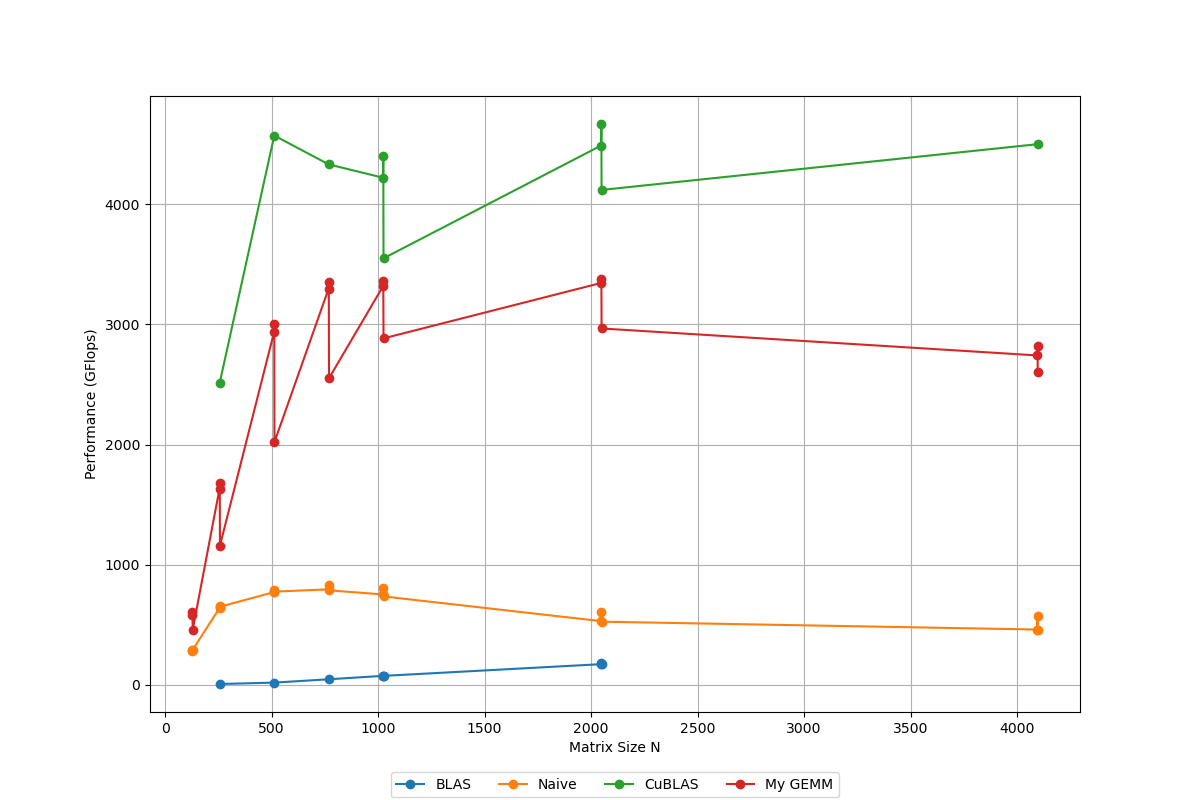
\includegraphics[width=\linewidth]{img/comparison.png}
    \caption{comparison}
    \label{fig:comparison}
\end{figure*}


\section{Analysis}

\subsection{comparison between methods}
Table \ref{tab:comparison} and Figure \ref{fig:comparison} shows the Peak GF of my GEMM program along with the performance from other implementations.

\subsection{curve shape}
As shown in Figure \ref{fig:comparison}, both my GEMM and the naive program suffered some performance loss on extra large matrix sizes,
The GF with $n=409$ is less than GF with $n=2048$.
However, CuBLAS is not affected by extra large matrix sizes.


\subsection{irregularities}
All non-naive implementation suffered performance loss 
on non-multiple matrix sizes, especially on $n=2^k+1$.
As the optimized program typically used partition to accelerate computation, and 
matrices with non-multiple sizes would cause some overhead.
Despite the performance loss on non-multiple matrix sizes compare to multiple matrix sizes, 
non-naive implementations are still faster than the native program at all matrices sizes.

\section{}
\subsection{}
$$
\begin{aligned}
\text{Peak Performance} 
    &= \text{SM Count} \times \text{Cores per SM} \times \text{Clock} \times \text{Ops per Cycle}\\
    &=40\times 64 \times 1.5G \times 2 \\
    &=7.68T
\end{aligned}
$$
To arrive the peak performance, the program's operation intensity (OI) should be 24.
The estimated OI of my program under theoretical memory bandwidth is 10.57.

\subsection{}
The estimated OI of my program under actual memory bandwidth is 15.37.
The estimated OI will increase as 
memory bandwidth decrease and the performance stay the same.

However the actual OI is inherit of program, 
and the estimation is based on the assumption that
the computation is either memory bounded or operation bounded,
i.e. the program is running on the roofline.

\begin{figure*}[h]
    \centering
    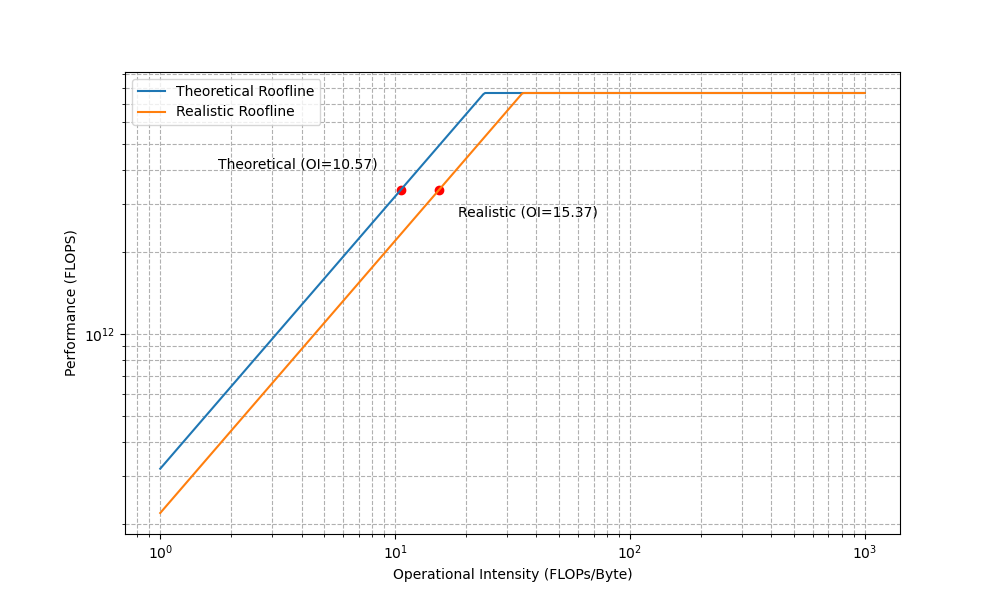
\includegraphics[width=\linewidth]{img/roofline.png}
    \caption{Theoretical and Realistic Roofline Model for NVIDIA T4 GPU}
    \label{fig:roofline}
\end{figure*}

\section{Potential Future Work}

Use Nvidia profiling tool to learn what other factors is limiting the computation, and if there is any improvement can be made.

\section{Extra Credits}
Implemented a non-square matrix multiplication kernel, 
that is able to take 2 matrices A and B of dimensions $M \times K$ and $K \times N$ respectively 
and compute C of $M \times N$. 

\begin{thebibliography}{9}
    \bibitem{cutlass_blog}
    NVIDIA. \textit{CUTLASS: Fast Linear Algebra in CUDA C++}.
    \url{https://developer.nvidia.com/blog/cutlass-linear-algebra-cuda/}.
    
    \bibitem{jia2019dissecting}
    Zhe Jia, Marco Maggioni, Jeffrey Smith, Daniele Paolo Scarpazza.
    \textit{Dissecting the NVIDIA Turing T4 GPU via Microbenchmarking}.
    \url{https://arxiv.org/pdf/1903.07486.pdf}.
    
\end{thebibliography}
\end{document}
